\documentclass[12pt,a4paper]{article}
\usepackage{placeins}
\usepackage[utf8]{inputenc}
\usepackage[ruled]{algorithm2e}
\usepackage{fullpage}
\usepackage{graphicx}
\usepackage{float}
\usepackage[portuguese]{babel}
\usepackage[]{amsmath}
\restylefloat{figure}

\usepackage[adobe-utopia]{mathdesign}
\usepackage[T1]{fontenc}

% \usepackage{mdframed}

\DeclareGraphicsExtensions{.jpg,.pdf}

\numberwithin{equation}{section}

\title{Trabalho Prático 3 - Expansor de Macros}
\author{Victor Pires Diniz}

\begin{document}
\maketitle
\begin{center}
Software Básico - 2º Semestre de 2015
\end{center}

\section{Descrição do trabalho}

O terceiro trabalho prático do semestre envolve o desenvolvimento de um expansor de macros para o código de montagem de uma máquina virtual especificada, para a qual foram feitos um emulador e um montador nos dois trabalhos prévios. O expansor de macros teria suporte a macros definidas em qualquer ponto no programa e instanciadas quantas vezes fosse necessário. Haveria, também, suporte a parâmetros, podendo haver um parâmetro ou nenhum. As macros poderiam ser instanciadas dentro de outras macros, mas não definidas.

Macros são uma forma simples e eficiente de abstração para o código de máquina, permitindo reutilização de código de forma relativamente flexível sem nenhum custo de desempenho em tempo de execução, visto que as macros são expandidas durante o processo de montagem.

\section{Implementação e decisões de projeto}

O código do expansor de macros está dividido semanticamente entre vários módulos:

\begin{itemize}
    \item \emph{main.c}: recebe parâmetros por linha de comando e chama o expansor de macros apropriadamente.
    \item Map (\emph{map.c, map.h, bucket.c, bucket.h}): implementa uma tabela de dispersão genérica, instanciada na tabela de macros.
    \item Função hash auxiliar (\emph{hash\_aux.c, hash\_aux.h}): contém uma função para hashing de string.
    \item Parser de linhas de código de montagem (\emph{line\_parser.c, line\_parser.h}): contém uma função que divide as linhas do código de montagem nos seus quatro elementos semânticos (label, operador e dois operandos).
    \item Funções auxiliares para strings (\emph{str\_aux.c, str\_aux.h}): contém duas funções para auxiliar no uso de strings ao longo do código.
    \item Vector (\emph{vector.c, vector.h}): implementa uma lista dinâmica de tipo único, utilizada na implementação da tabela de macros.
    \item Tabela de macros (\emph{macro\_table.c, macro\_table.h}): tipo onde as macros são armazenadas e, posteriormente, de onde elas são instanciadas. Realiza a substituição de parâmetros e o tratamento das labels definidas dentro das macros.
    \item Expansor (\emph{expander.c, expander.h}): módulo principal do expansor de macros. Define a função principal do programa e, internamente, realiza as duas passadas do expansor de macros.
\end{itemize}

Os mais importantes deles serão analisados a seguir em mais detalhe.

\subsection{Map}

O módulo map contém a implementação de uma hash table totalmente genérica, com tratamento de colisão através de listas encadeadas, definidas nos arquivos \emph{bucket.c} e \emph{bucket.h}.

\subsection{Vector}

Este módulo implementa uma lista genérica dinamicamente alocada para armazenar as linhas de código de montagem das macros. A implementação dessa lista é feita de maneira contígua, com um vetor interno à estrutura. Esse vetor é expandido dinamicamente conforme necessário, crescendo exponencialmente (por um fator de 1,5) sempre que o número de elementos alcança o número máximo de elementos do vetor.

\subsection{Tabela de macros}

A tabela de macros é um módulo essencial para o funcionamento deste expansor, interagindo diretamente com o processo de expansão. Além das funções de inicialização e finalização (\emph{mtCreate} e \emph{mtDestroy}, respectivamente), o módulo disponibiliza duas funções principais: inserção e avaliação.

A tabela de macros em si consiste em um Map de strings para um tipo \emph{Macro}, definido internamente. Esse tipo contém as informações importantes a serem guardadas sobre as macros definidas: o conteúdo textual de cada uma armazenado num \emph{Vector} de strings, o nome do seu parâmetro a ser substituído (opcional), o número de vezes que a macro foi instanciada no programa e um Map que armazena as labels definidas dentro da macro.

\emph{mtInsert}, a função de inserção, tem funcionamento simples: ela apenas insere a macro nova no Map interno à tabela de macros. A função \emph{mtEval}, porém, é mais complexa. Essa função é responsável por avaliar a macro, substituir o seu parâmetro pelo parâmetro da instanciação em questão, adicionar um sufixo às labels definidas internamente para evitar conflitos e retornar uma string que contenha essa macro. Antes disso, ocorre uma etapa de pré-processamento, caso a macro esteja sendo invocada pela primeira vez. Isso se deve à possibilidade de instanciação de macros dentro de macros: após o pré-processamento, o conteúdo do vetor da macro contém as versões expandidas das suas macros internas. Depois disso, são substituídos os termos citados e a função retorna a string com a macro pronta para uso no código de montagem.

\subsection{Expansor}

O expansor de macros opera em dois passos principais. O primeiro deles, desempenhado na função \emph{buildMacroTable}, consiste em passar pelo código de montagem em busca de macros, registrando o conteúdo de cada uma na tabela de macros. 

Ao passar pela segunda vez, com a função \emph{replaceAndOutput}, a expansão real é realizada, imprimindo para o arquivo de saída o código de montagem obtido com a expansão das macros. Definições de macro são completamente ignoradas, visto que elas já foram processadas anteriormente, e linhas de código que não contém macros ou definições são impressas intactas.

\section{Compilação e execução}

A compilação do expansor de macros pode ser realizada através da \emph{makefile} disponibilizada ou diretamente através do \emph{GCC} ou outro compilador C. Caso compilado através da \emph{makefile}, o executável estará localizado na pasta \verb|bin/|. A execução do programa deve ser realizada através da linha de comando, na seguinte forma,

\begin{verbatim}
    {endereço do executável do expansor} <input_addr> <output_addr>
\end{verbatim}

em que:

\begin{itemize}
    \item \verb|input_addr|: endereço para o arquivo de entrada, em código de montagem.
    \item \verb|output_addr|: endereço para o arquivo de saída a ser criado.
\end{itemize}

\section{Testes realizados}

Na pasta de testes presente no pacote deste trabalho, há diversos programas que foram utilizados para garantir o bom funcionamento do expansor de macros, cobrindo diversas formas de instanciação e definição de macros no programa. Vários deles foram implementados de acordo com o pedido na especificação do trabalho. Imagens da execução dos testes estão disponíveis no apêndice desta documentação. Segue abaixo uma breve descrição do comportamento de cada programa:

\begin{itemize}
    \item \verb|tfat.i|: Calcula o fatorial de um número natural. \emph{Pedido na especificação do trabalho.}
    \item \verb|tmdc.i|: Calcula o MDC de dois números inteiros. \emph{Pedido na especificação do trabalho.}
    \item \verb|tspec0.i|: Imprime o maior valor entre dois inteiros. \emph{Disponibilizado na especificação do trabalho.}
    \item \verb|tspec1.i|: Testa funcionalidade do expansor para macros sem parâmetros, gera código de montagem inválido. \emph{Disponibilizado na especificação do trabalho.}
    \item \verb|tspec2.i|: Testa funcionalidade do expansor para macros com parâmetros, gera código de montagem inválido. \emph{Disponibilizado na especificação do trabalho.}
\end{itemize}

\subsection{Testes unitários}

Além das entradas de teste elaboradas, foram criados também diversos \emph{unit tests}, com o propósito de testar a funcionalidade de cada módulo do expansor de macro. Esses testes estão disponíveis na pasta \verb|unit-tests/|, dentro da pasta de testes, e podem ser compilados com o comando \verb|make tests|, que utiliza uma funcionalidade adicional da \emph{makefile} providenciada. Após a compilação, eles estarão localizados na pasta \verb|bin/test-bin/|.

\section{Conclusão}

Neste trabalho, foi implementado um expansor de macro para uma máquina virtual, definido de acordo com a especificação fornecida. O comportamento e a implementação do expansor de macro foram discutidos no contexto dos testes realizados e da interação com o emulador criado no trabalho prático anterior, de forma a garantir que as instruções e pseudo-instruções funcionam como previsto.

% \appendix

% \section{Imagens de execução dos testes}

% \begin{figure}[h]
%     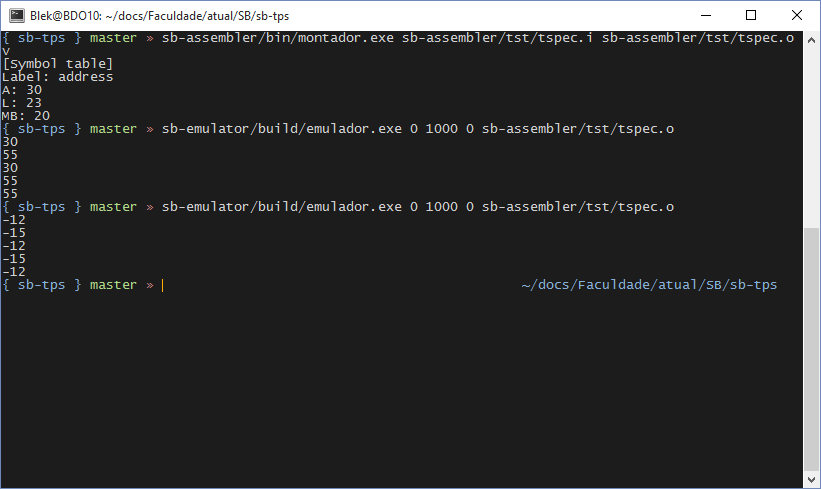
\includegraphics[scale=0.7]{imagens/tspec_console.png}
%     \centering
%     \caption{Montagem em modo verboso e execução do teste tspec.i.}
% \end{figure}

% \begin{figure}[h]
%     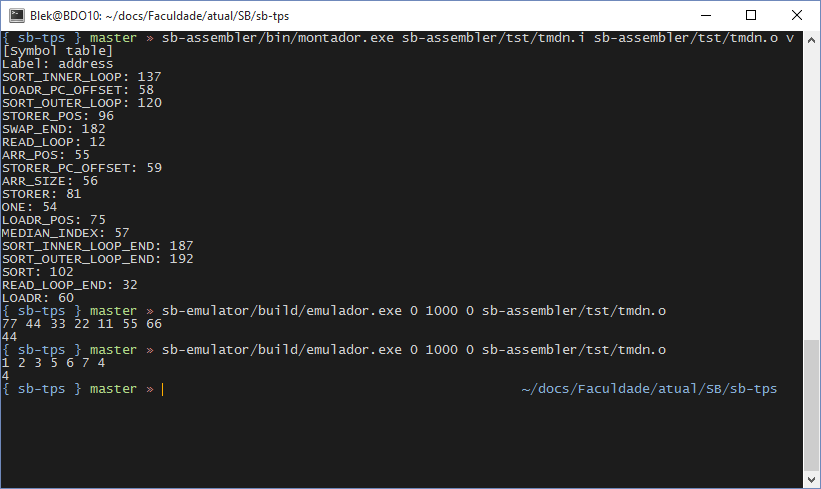
\includegraphics[scale=0.7]{imagens/tmdn_console.png}
%     \centering
%     \caption{Montagem em modo verboso e execução do teste tmdn.i.}
% \end{figure}

% \begin{figure}[h]
%     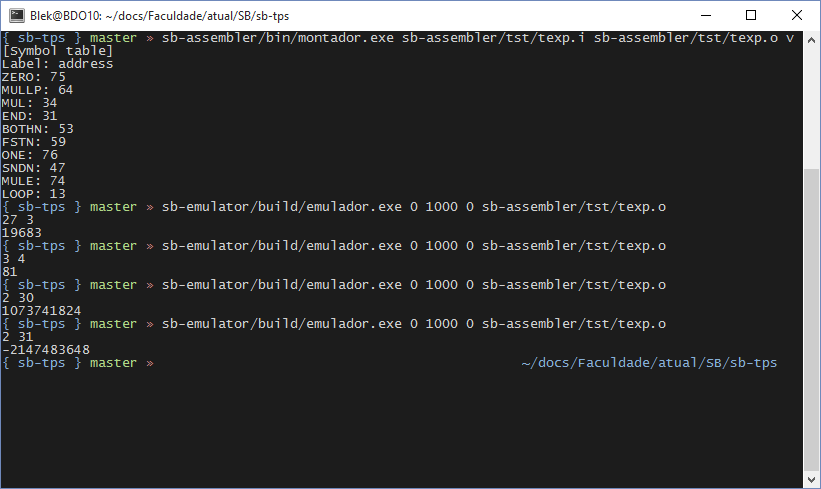
\includegraphics[scale=0.7]{imagens/texp_console.png}
%     \centering
%     \caption{Montagem em modo verboso e execução do teste texp.i.}
% \end{figure}

% \begin{figure}[h]
%     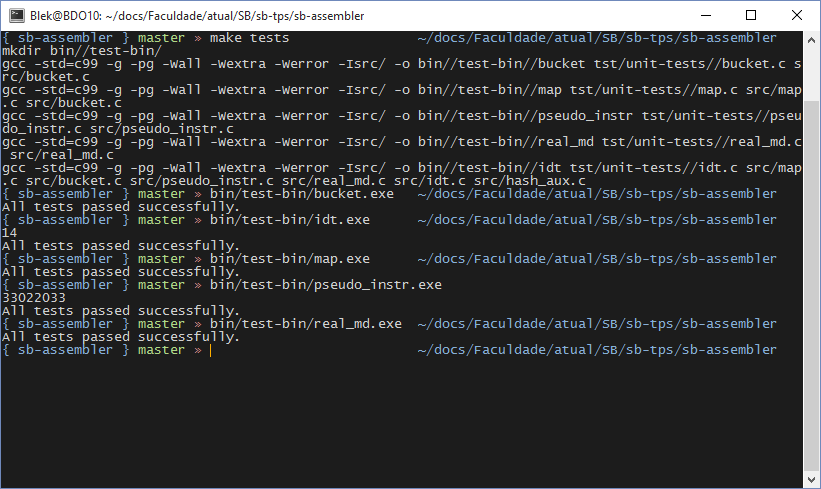
\includegraphics[scale=0.7]{imagens/unit_tests_console.png}
%     \centering
%     \caption{Compilação e execução dos testes unitários providenciados.}
% \end{figure}

% \FloatBarrier

\end{document}